\section{Past Similar Projects}

Medical imaging for the purposes of volume reconstruction, body size/feature estimation or markerless recognition has seen widespread research and commercial application. This includes the use of MRI scanners that use frequencies outside of the visible spectrum for the production of volume images to the use of conventional cameras for the monitoring of surface movement or for the profiling of a patient. The PARSE project aims to combine some of these elements into a platform that uses range imaging technology in the form of a Microsoft Kinect. There are similar noteworthy projects which have been identified below as a sound basis for our work with the Kinect and associated methodologies. \\

\subsection{Profiling a Surface}

Structured Light provides a reliable way in which to capture and recover object surfaces using a projector-camera configuration. Currently, to give an accurate profilometry of a surface that can be reconstructed and produce a reasonable volume result, the surface needs to be dense and have reasonable correspondence between repeated scans in a defined configuration. Salvi et al through their analysis of structured light techniques evaluated the effectiveness of Coded (coloured) structured light for the discrete coding of objects that produced an accurate surface profile \cite{Salvi2010}. Instead of traditional air displacement plethysmography, surface profilometry computer vision techniques can be used in a form of structured light plethysmography. It's current usage is in pulmonary function testing where a 3D reconstruction is generated from projection, scan and capture of the chest area during normal or regulated breathing activity \cite{DeBoer2010}. The structured light approach is noted as being non-invasive and has the benefit of being markerless as positioning of the scanner relative to the body can be stored electronically and tracked over time as the patient's condition or composition changes. \\

%A state of the art in structured light patterns for surface profilometry (http://www.sciencedirect.com/science/article/pii/S003132031000124X)

%not sure about this one...

%\subsection{Monitoring Facial Surface Change}

%Quantification of Facial Surface Change Using a Structured Light %Scanner (http://journals.lww.com/plasreconsurg/abstract/1994%%%/11000/quantification_of_facial_surface_change_using_a.3.aspx)

\subsection{Estimating Patient Size}

%Using the Microsoft Kinect for Patient Size Estimation and Radiation Dose Normalization: Proof of Concept and Initial Validation (http://link.springer.com/article/10.1007/s10278-012-9567-2/fulltext.html)

Estimating patient size is important for the idenfication of radiation dosage. Smaller patients are likely to be more sensitive to radiation exposure compared to older, larger subjects \cite{McCollough2011}. In this project, the authors used the Kinect in a configuration where only the depth map and weight of the patient was captured. The use of the depth map was then extrapolated to the rear of the patient and a coarse volume calculated using a convex hull algorithm \cite{Cook2013}. Other factors such as gender and age were kept anonymous as the authors wished to examine the effect of the person's pose configuration on their volume. In particular, different arm configurations (extended or across the chest) yielded greatly different volumes registered by the Kinect compared to the default configuration and hence the radiation dosage to be administered. \\

\begin{figure}[htb]
\begin{center}
    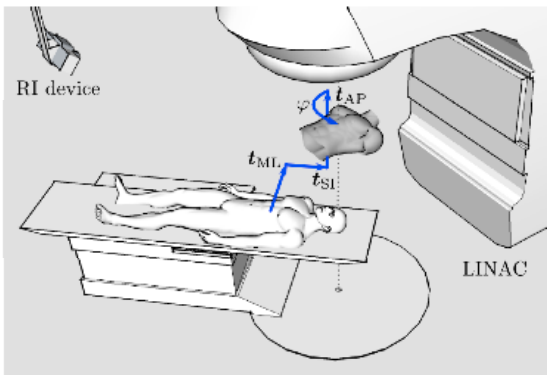
\includegraphics[scale=0.5]{images/celingkinectconfig.PNG}
    \caption{A celing mounted Kinect for the purposes of calibrating patients for CT scanning.}
\end{center}
\end{figure}

Interestingly, the authors suggest that the use of additional Kinect devices or alternative scanning configuration in this instance would provide more accurate and consistent volume measurement. An addendum to the further work possible is the use of the Kinect as a celing-mounted volume estimation pre-requisite before a patient undergoes CT scanning so that the appropriate radiation dosage is administered. Additionally, an implementation that is able to take account of positional differences/angles and calculate volume more robustly as a result is considered.

\subsection{Visual Weight Estimation}

Estimating weight using conventional computer vision techniques has traditionally relied on complex classification methods for the determination of particular parts of the body. In space, the context in which measuring the mass of a person does not have the luxury of a constant gravity for traditional methods, Verlado and Dugelay \cite{Veraldo2012} devised a system that used the offline labelling and determination of anthropometric measures to estimate overall body mass using linear regression methods. Work by Paleria and Araino \cite{Paleria2011} aimed to improve upon anthropometric identification and mass calculation with the additional identification of gender and age which influences the overall mass of a person and their siri ratio using machine learning methods such as neural networks to determine these variables. \\

The Kinect is used to take the labelling of anthropometric measures \emph{online} and hence using the NITE framework\footnote{The `standard' framework for 3D Sensing, \emph{http://www.openni.org/}} included in the API of the software, identify and track these areas of the body. The weight of the person is estimated by computing the lengths of the limbs and calculating their relevant circumferences, applying a median filter over repeated measures to reduce the influence of the offset, or shadowing, produced by the 3D sensor. The presence of noise due to sensor flickering or subject movement is considered and extrapolation factors, calculated through repeated trials, is suggested for the more accurate measurement and representation of circumferences for the arms, legs and waist.\\

Veraldo and Dugelay are able to calculate the weight determined by the Kinect sensor by utilising a statistical model trained on a large medical database of anthropometric measures that returns accurate mass representations of queried limbs within a certain tolerance, +/- 2.7cm typically for arm circumference measurement \cite{Paleria2011}. Access to a medical database of such size isn't feasible in this project and our concern with the calculation of volume and limb circumference rather than mass directly means the project could easily make use of a model with little additional development overhead. \\

\subsection{Whole Body Scanning}

One area which has seen particular development concentration is the concept of 3D Body scanning for rapid prototyping of avatars and for the purposes of editing and sharing of 3D models in specialised modelling applications such as Autodesk. Cui et al have designed a scanning pipeline and kinect configuration which is able to generate 3D models from Kinect Input data and utilise super-resolution, a class of techniques that can be used to improve the resolution of an imaging system, to improve the resolution of the Kinect images. The have also utilised a non-rigid method of registration between captured point clouds to form an accurate visual representation of the scanned subject \cite{Cui2012}. Unlike some body scanning implementations, Cui et al use a configuration which requires the subject to rotate 360\degree on the spot in a 'T' position. Registration between frames is calculated using a maximum-likelihood formulation and iterative expectation maximization to align scans based on probabilistic examination of correspondence between their points. The model is then rendered using a textured depth map. There are an increasing number of commercial and open source applications, particularly through the OpenNI \cite{openNi13} initiative which are using range imaging for full scale body rendering. \\
